\chapter{TESTING DOCUMENTATION}
\label{appen:b}

\section*{COMPONENT TESTING AND CALIBRATION}

\begin{figure}[H]
	\centering
	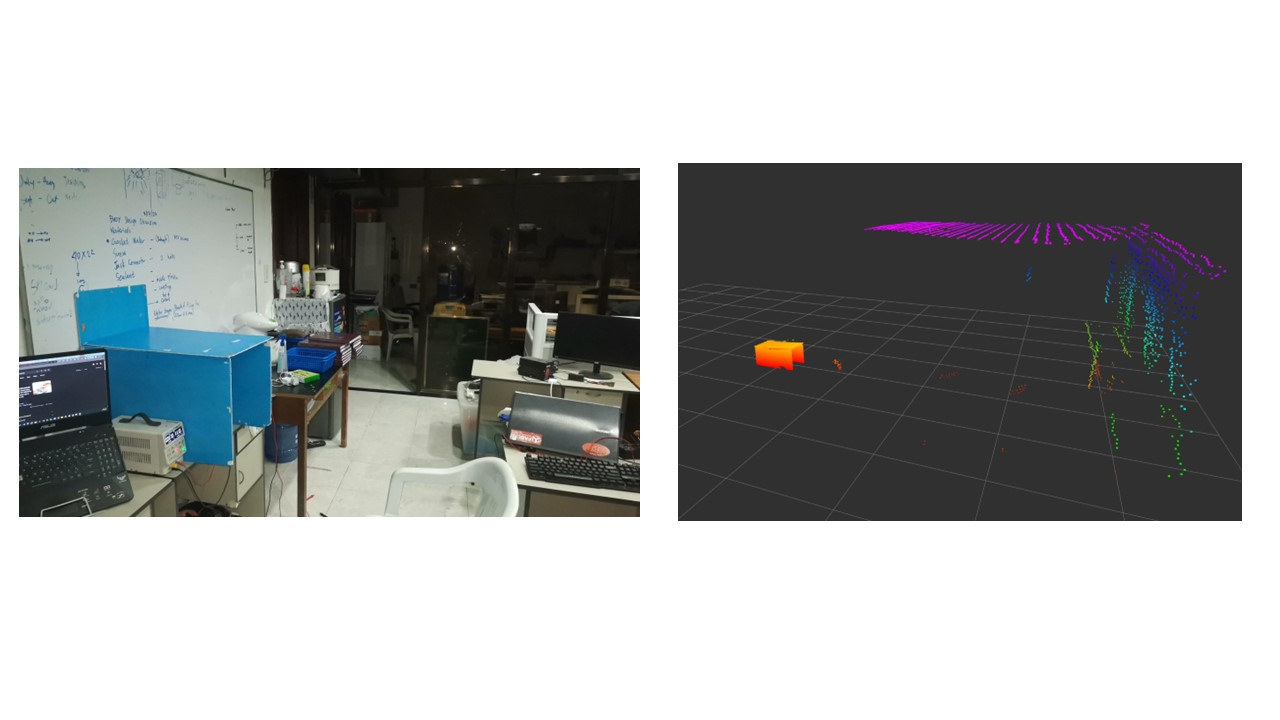
\includegraphics[width=0.9\textwidth]{Figures/Appendecis/testing/Slide1}
	\caption*{3D Point Cloud Calibration (Laboratory Testing)}
\end{figure}

\begin{figure}[H]
	\centering
	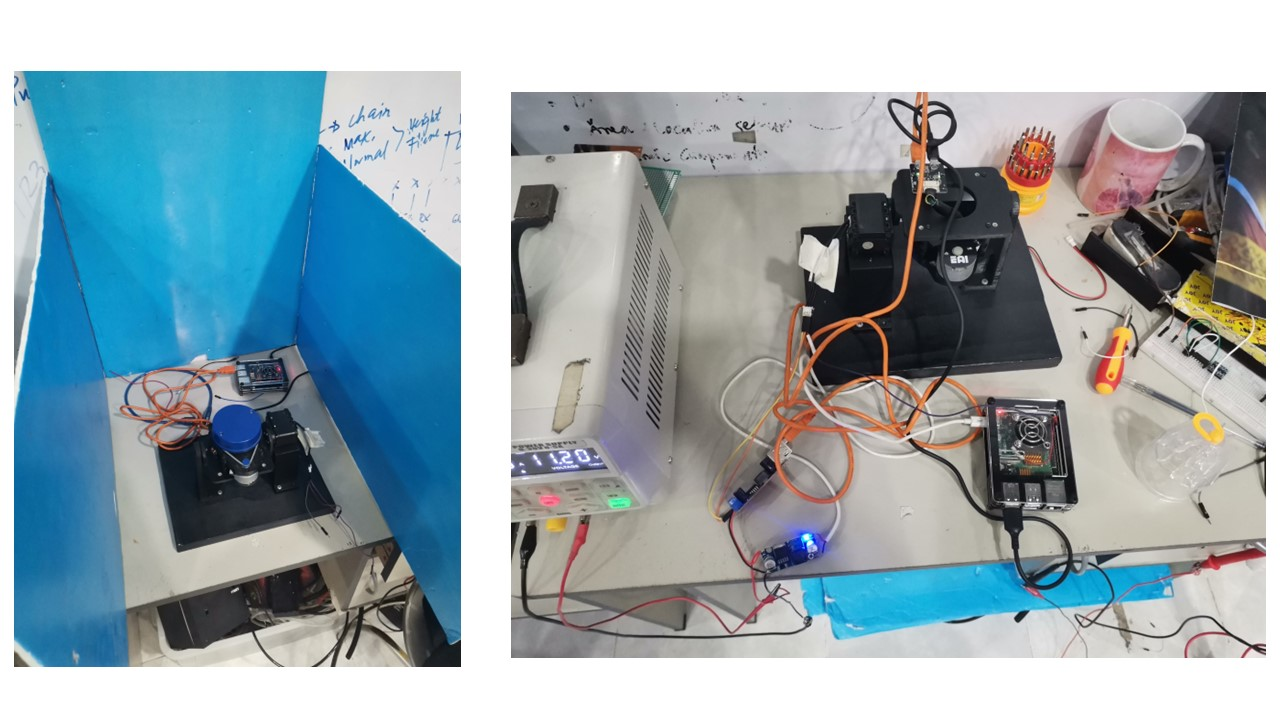
\includegraphics[width=0.8\textwidth]{Figures/Appendecis/testing/Slide2}
	\caption*{Actual Servo Calibration}
\end{figure}

\newpage

\begin{center}
	\textbf{APPENDIX B (Contd.)}
\end{center}

\begin{figure}[H]
	\centering
	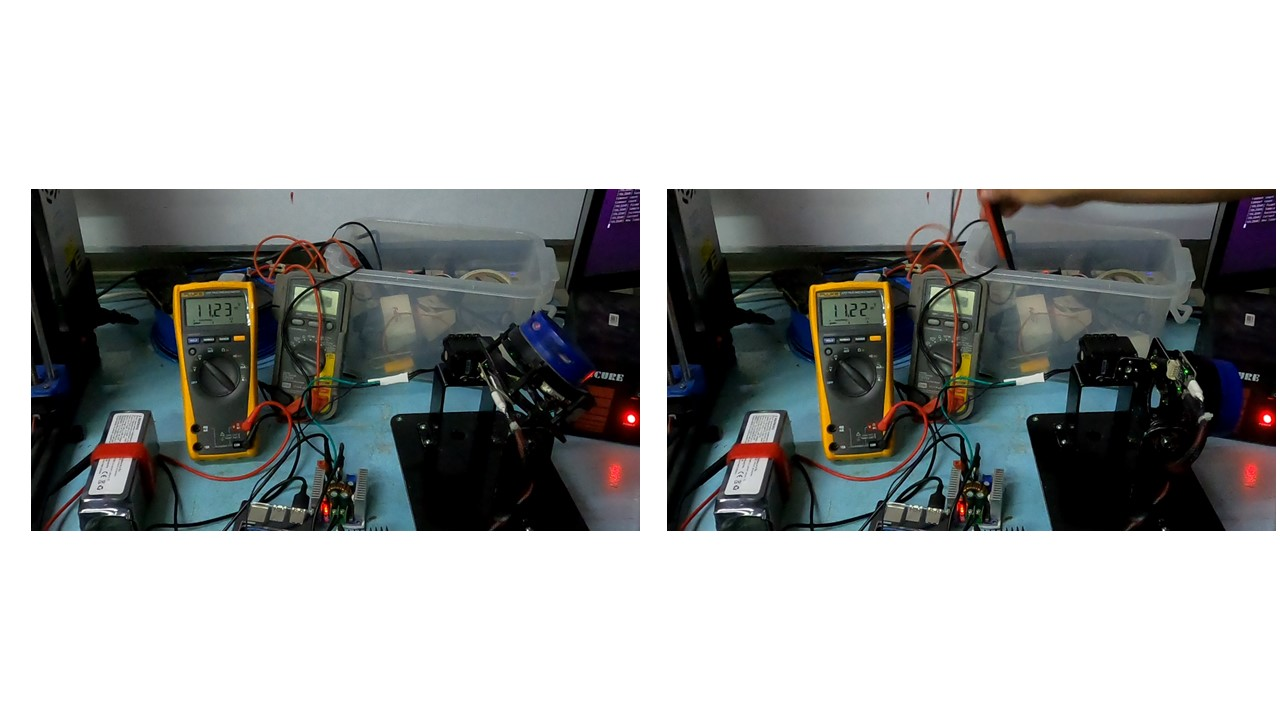
\includegraphics[width=1\textwidth]{Figures/Appendecis/testing/Slide3}
	\caption*{3D Point Cloud Calibration (Contd.)}
\end{figure}
\begin{figure}[H]
	\centering
	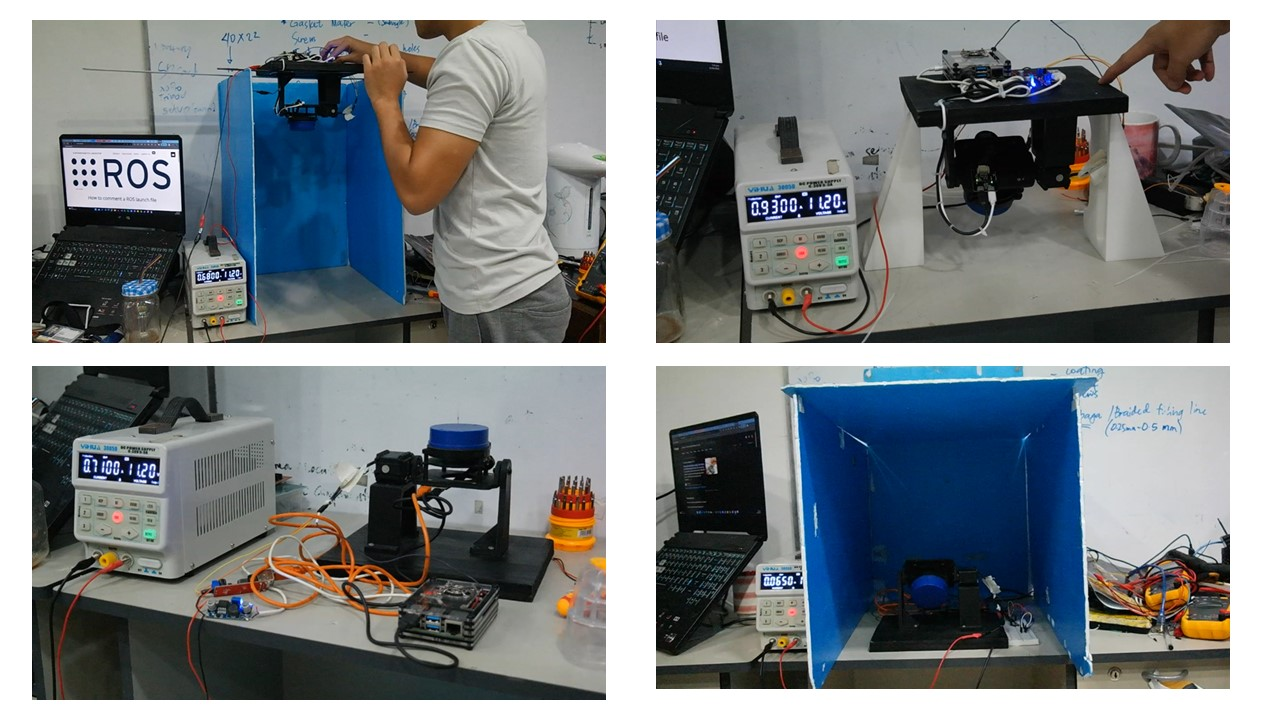
\includegraphics[width=1\textwidth]{Figures/Appendecis/testing/Slide4}
	\caption*{3D Point Cloud Calibration (Contd.)}
\end{figure}

\newpage

\begin{center}
	\textbf{APPENDIX B (Contd.)}
\end{center}

\section*{ACTUAL TESTING}

\begin{figure}[H]
	\centering
	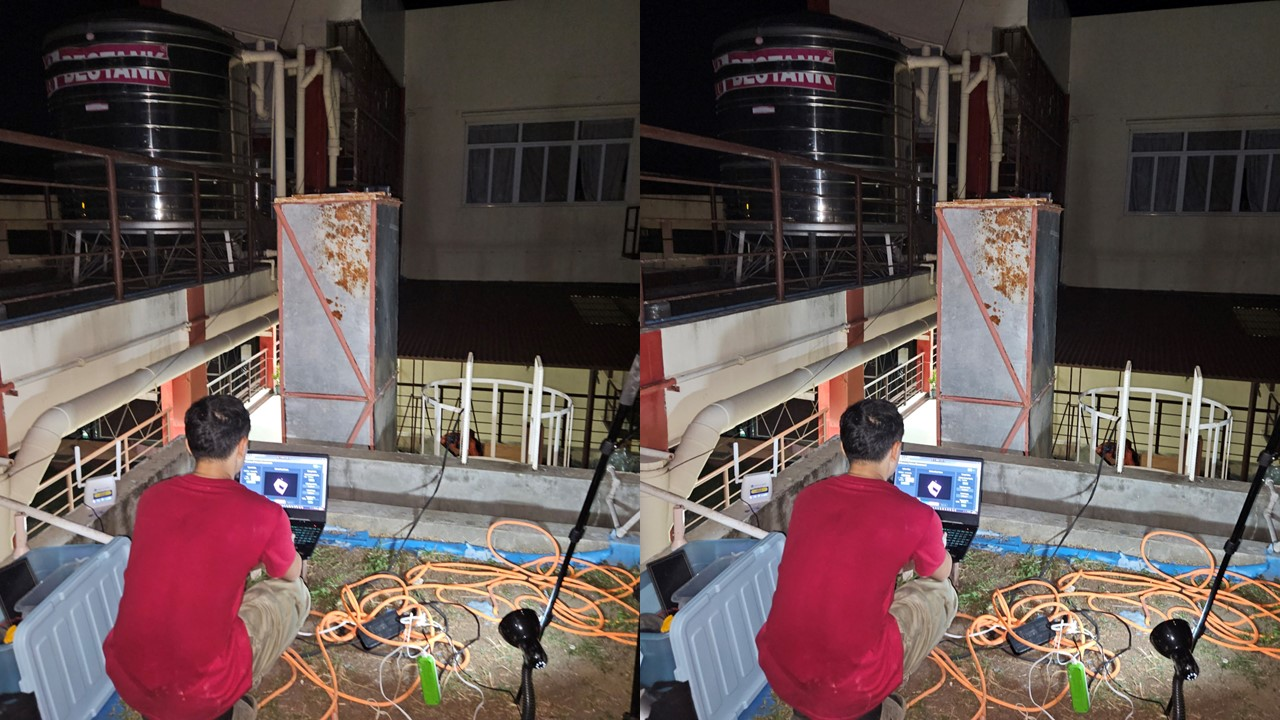
\includegraphics[width=1\textwidth]{Figures/Appendecis/testing/Slide5}
	\caption*{Actual Storage Bin Testing with the System}
\end{figure}
\begin{figure}[H]
	\centering
	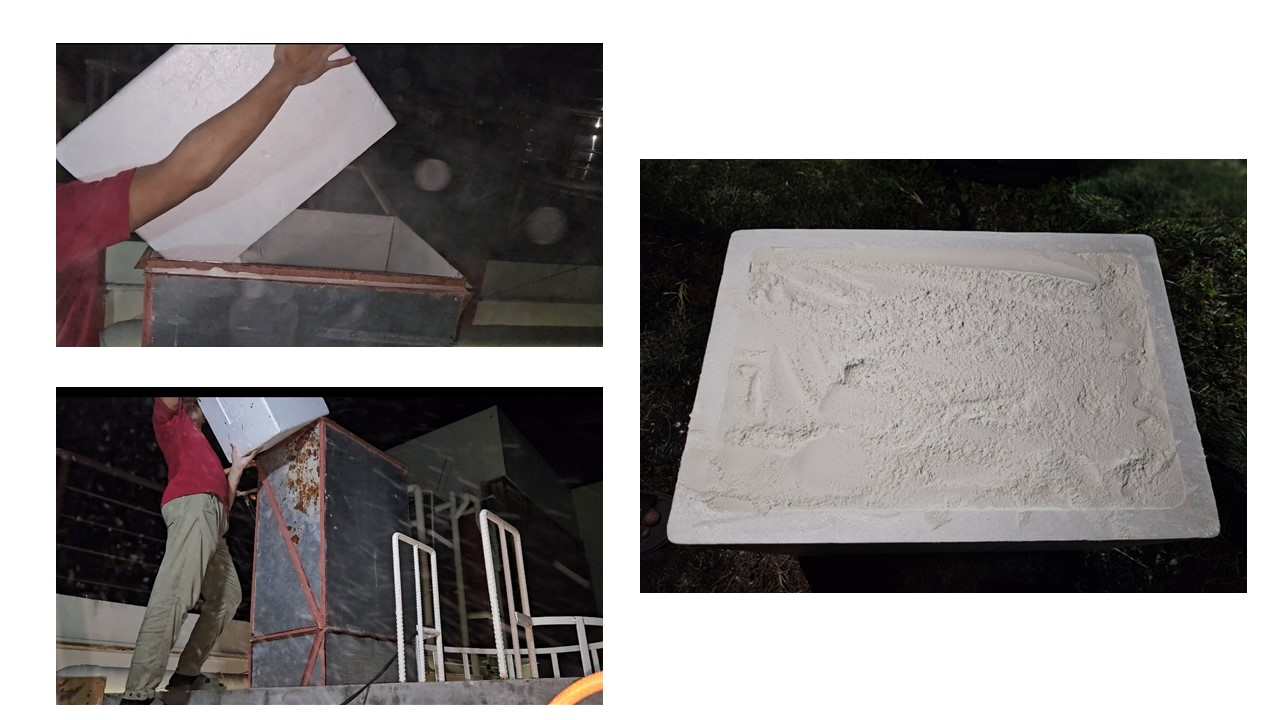
\includegraphics[width=1\textwidth]{Figures/Appendecis/testing/Slide6}
	\caption*{Actual Filling of Flour with Known Volume}
\end{figure}

\newpage

\begin{center}
	\textbf{APPENDIX B (Contd.)}
\end{center}
\begin{figure}[H]
	\centering
	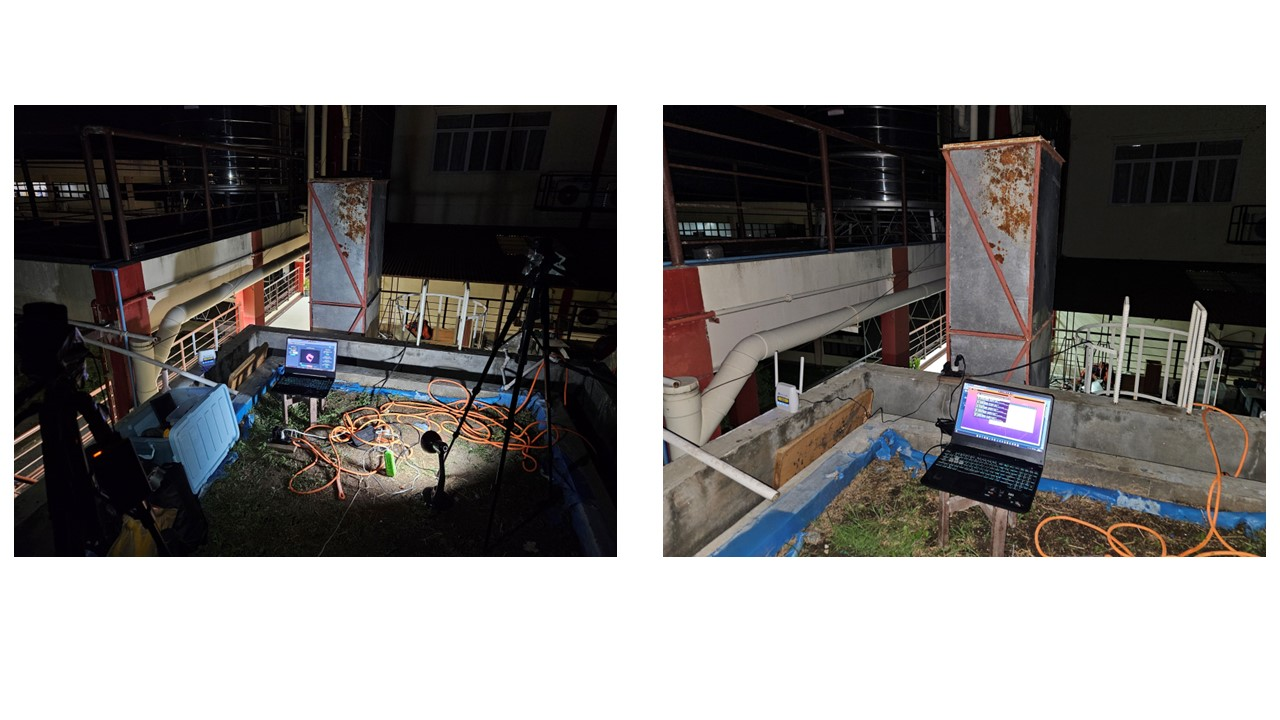
\includegraphics[width=1\textwidth]{Figures/Appendecis/testing/Slide7}
	\caption*{Actual Testing Site}
\end{figure}
\begin{figure}[H]
	\centering
	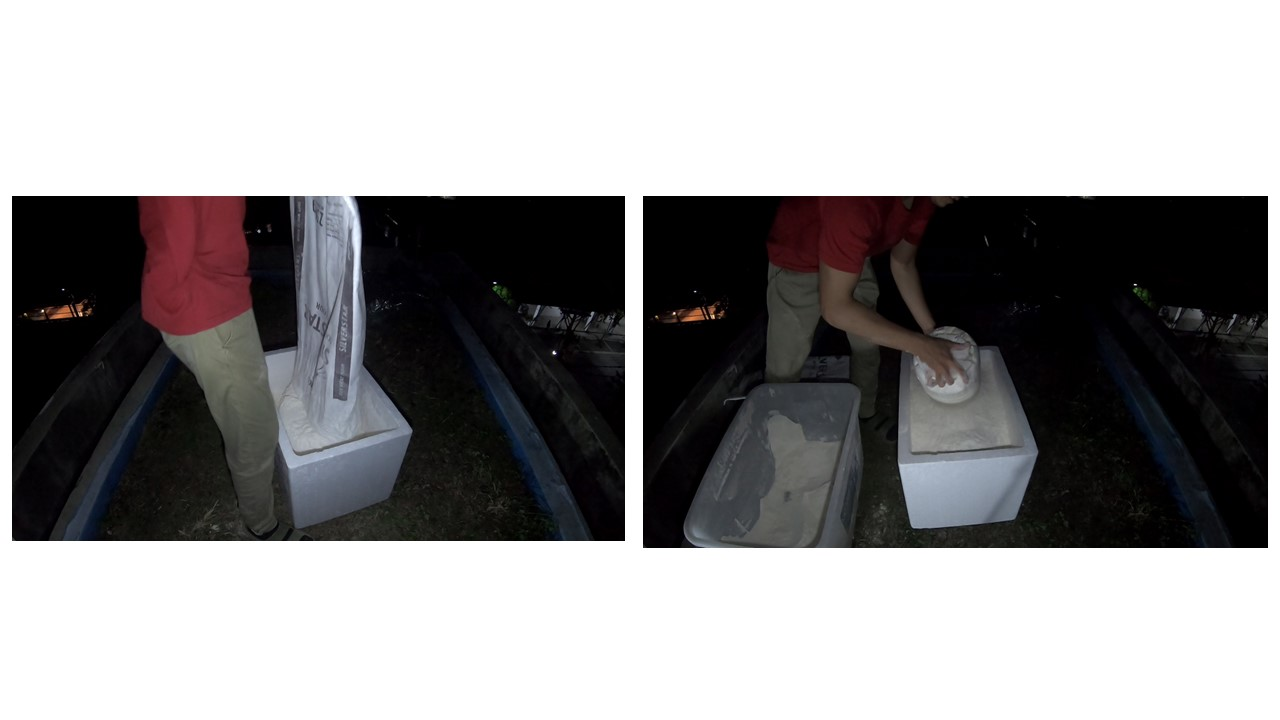
\includegraphics[width=1\textwidth]{Figures/Appendecis/testing/Slide8}
	\caption*{Known Volume}
\end{figure}

\newpage

\begin{center}
	\textbf{APPENDIX B (Contd.)}
\end{center}
\begin{figure}[H]
	\centering
	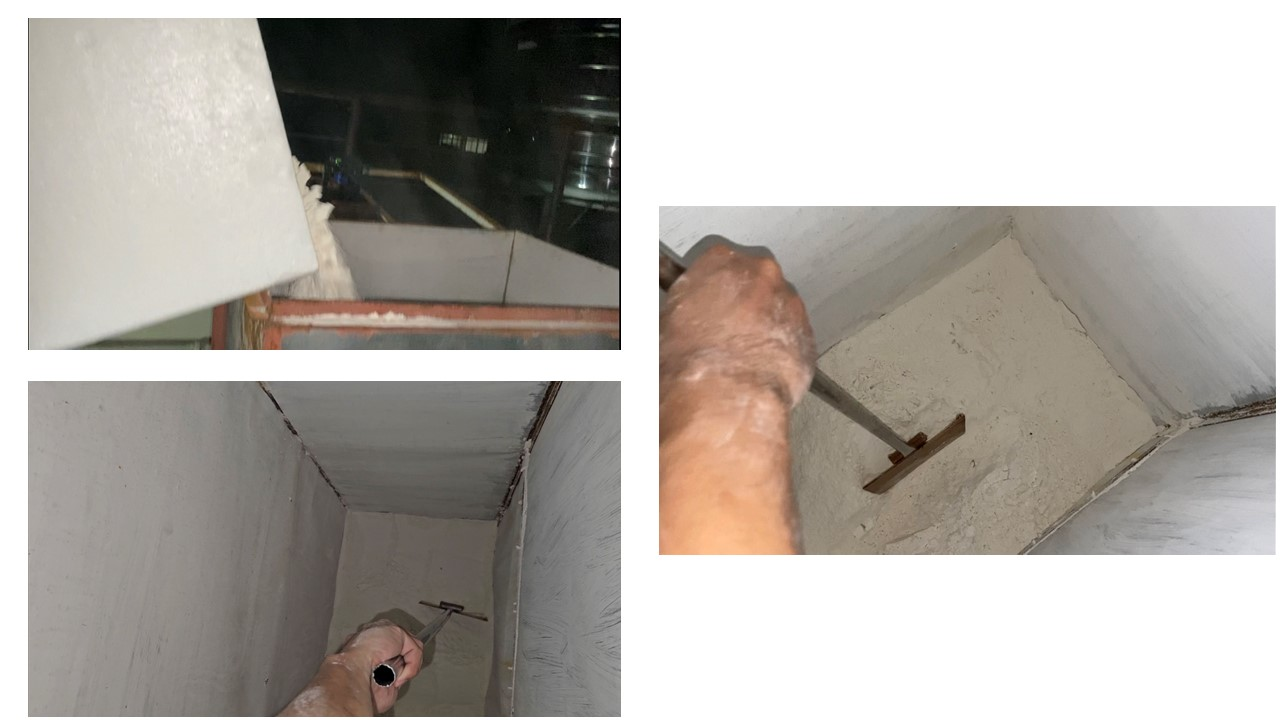
\includegraphics[width=1\textwidth]{Figures/Appendecis/testing/Slide9}
	\caption*{Actual Changing of Contour}
\end{figure}
\begin{figure}[H]
	\centering
	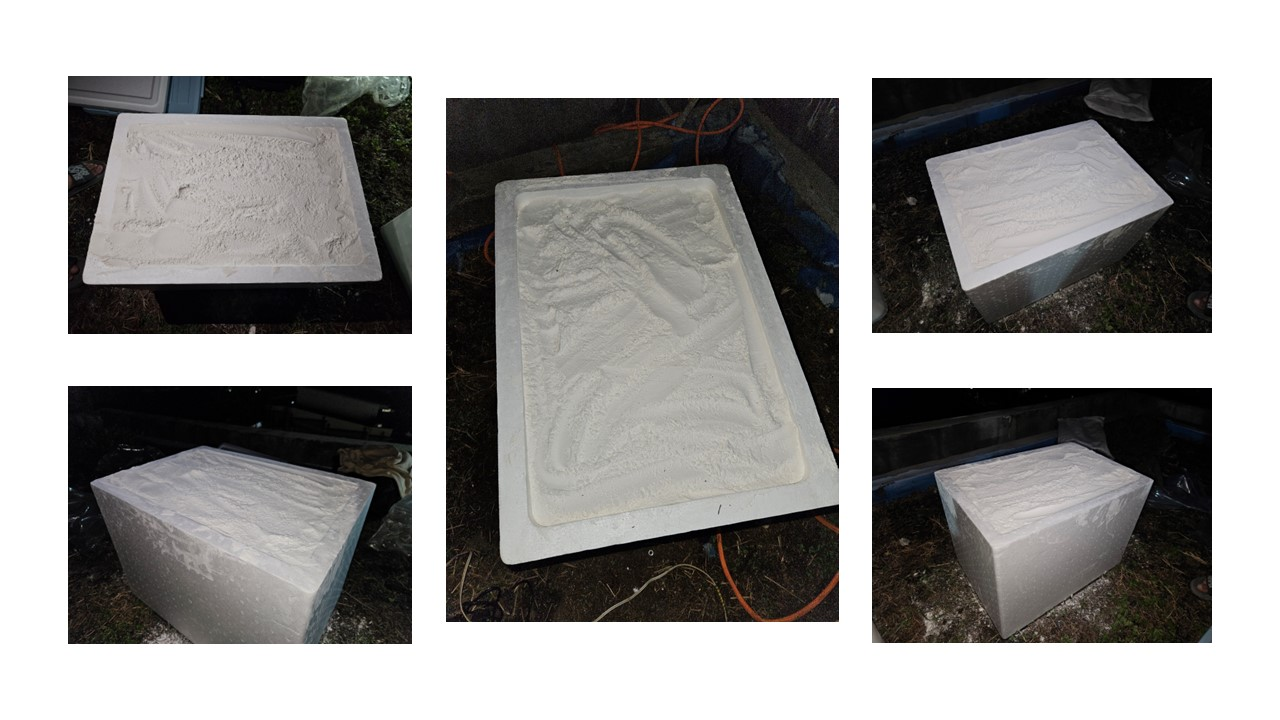
\includegraphics[width=1\textwidth]{Figures/Appendecis/testing/Slide10}
	\caption*{Actual Known Volume}
\end{figure}

\newpage

\begin{center}
	\textbf{APPENDIX B (Contd.)}
\end{center}

\begin{figure}[H]
	\centering
	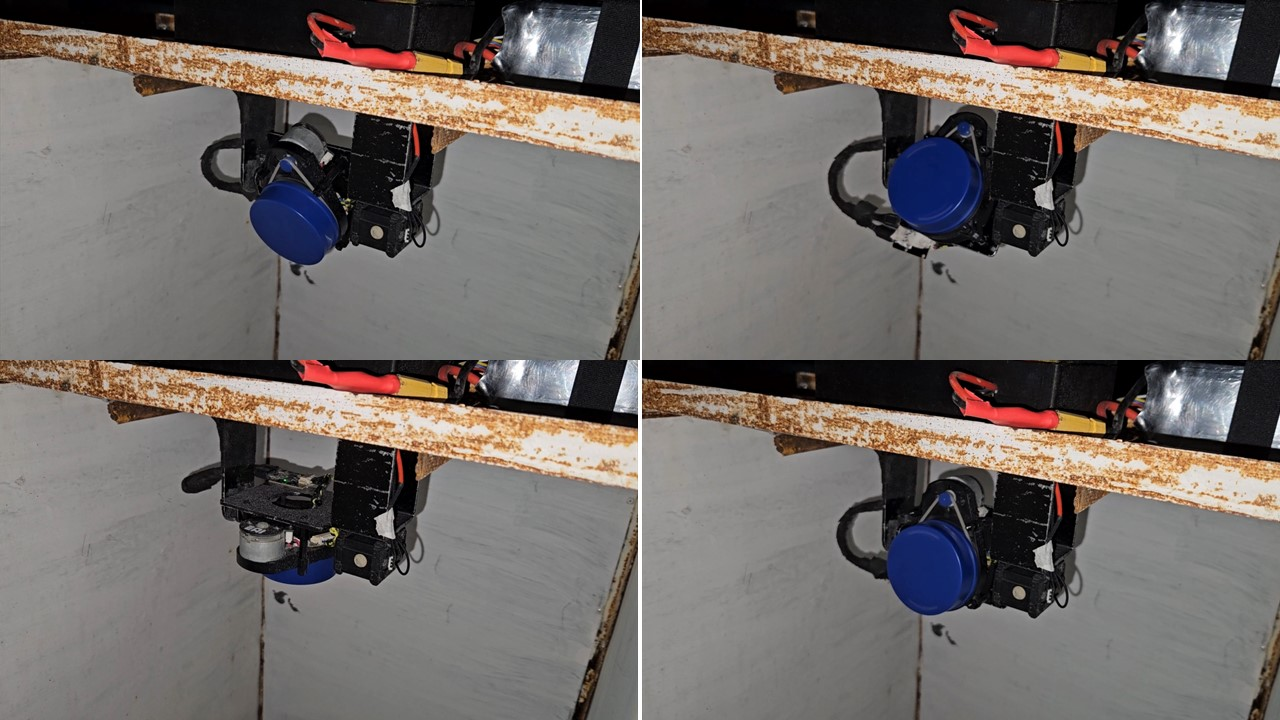
\includegraphics[width=1\textwidth]{Figures/Appendecis/testing/Slide12}
	\caption*{The 3D Point Cloud Scanner System Actual Operating}
\end{figure}

\begin{figure}[H]
	\centering
	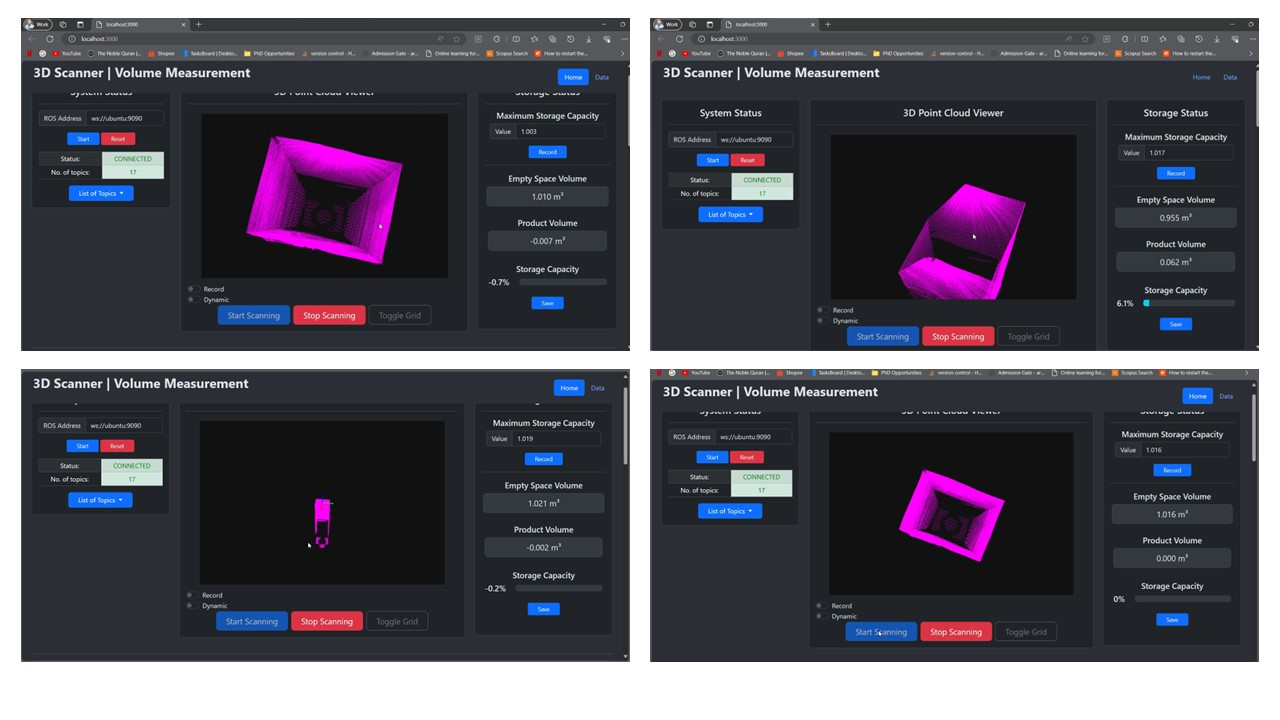
\includegraphics[width=1\textwidth]{Figures/Appendecis/testing/Slide11}
	\caption*{Web Application During Scanning}
\end{figure}

\newpage
\begin{center}
	\textbf{APPENDIX B (Contd.)}
\end{center}
\section*{System and Sounding Method Actual Testing}

\textbf{CONTOUR 1}

\begin{figure}[H]
	\centering
	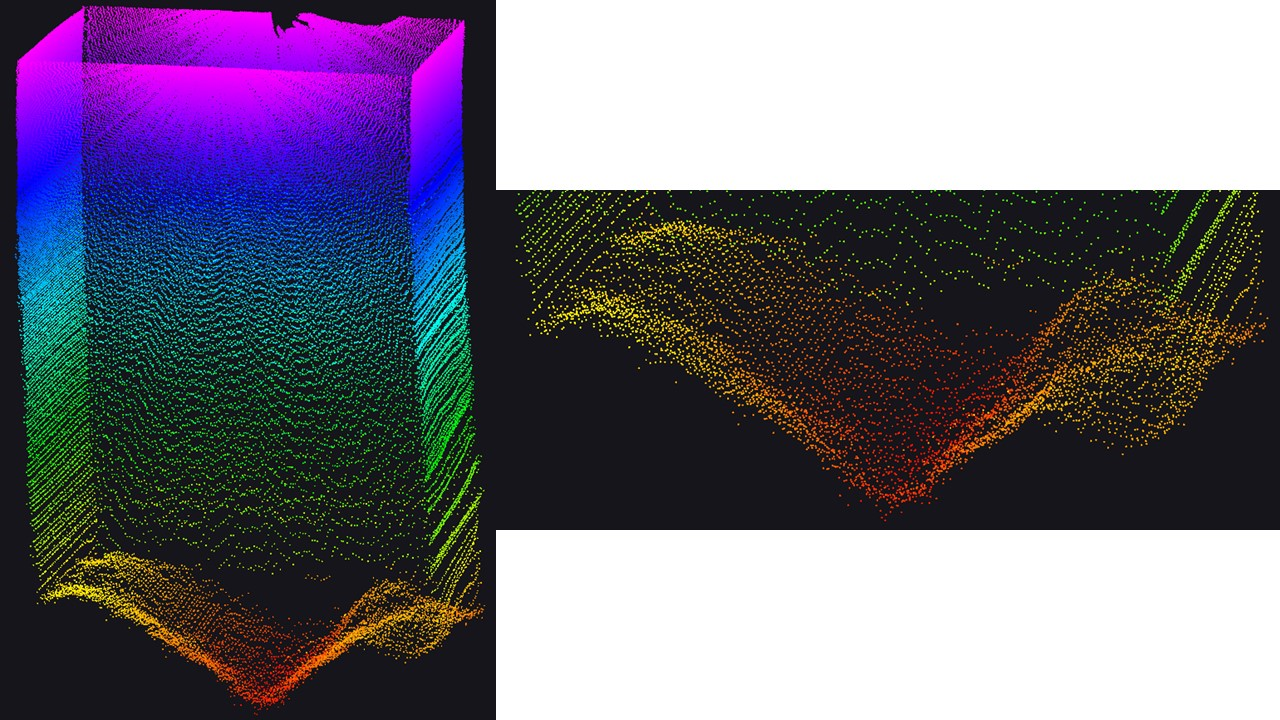
\includegraphics[width=1\textwidth]{Figures/test3-1}
	\caption*{3D Point Cloud of Contour 1}
\end{figure}

\vspace{0.5cm}

\begin{figure}[H]
	\centering
	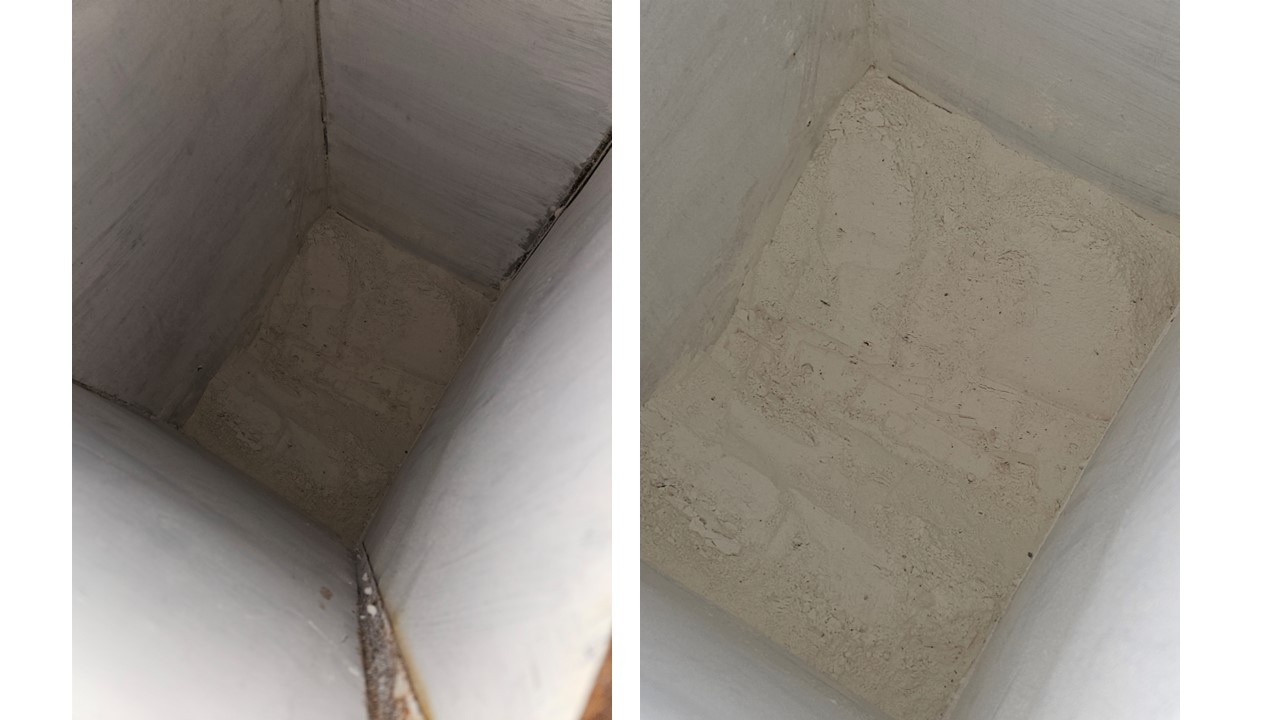
\includegraphics[width=1\textwidth]{Figures/test3-1-actual}
	\caption*{Actual Contour of 1}
\end{figure}

\newpage

\begin{center}
	\textbf{APPENDIX B (Contd.)}
\end{center}

\textbf{CONTOUR 2}

\begin{figure}[H]
	\centering
	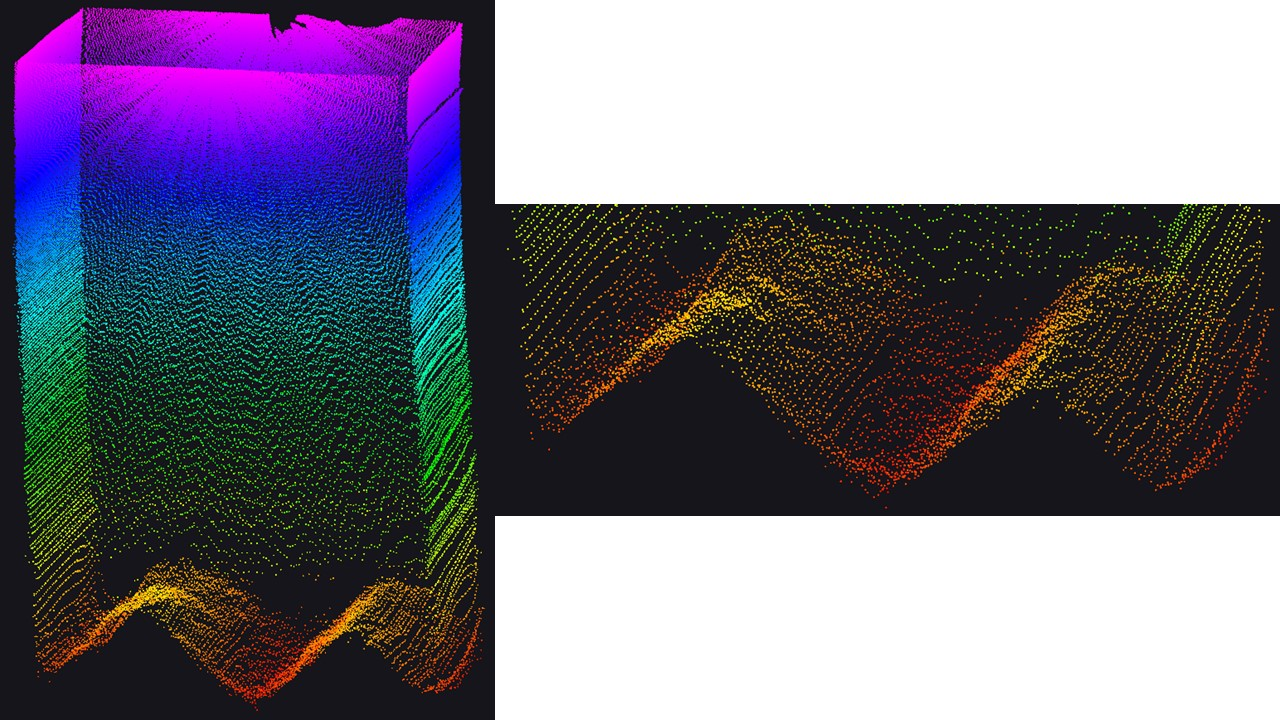
\includegraphics[width=1\textwidth]{Figures/test3-2}
	\caption*{3D Point Cloud of Contour 2}
\end{figure}

\vspace{0.5cm}

\begin{figure}[H]
	\centering
	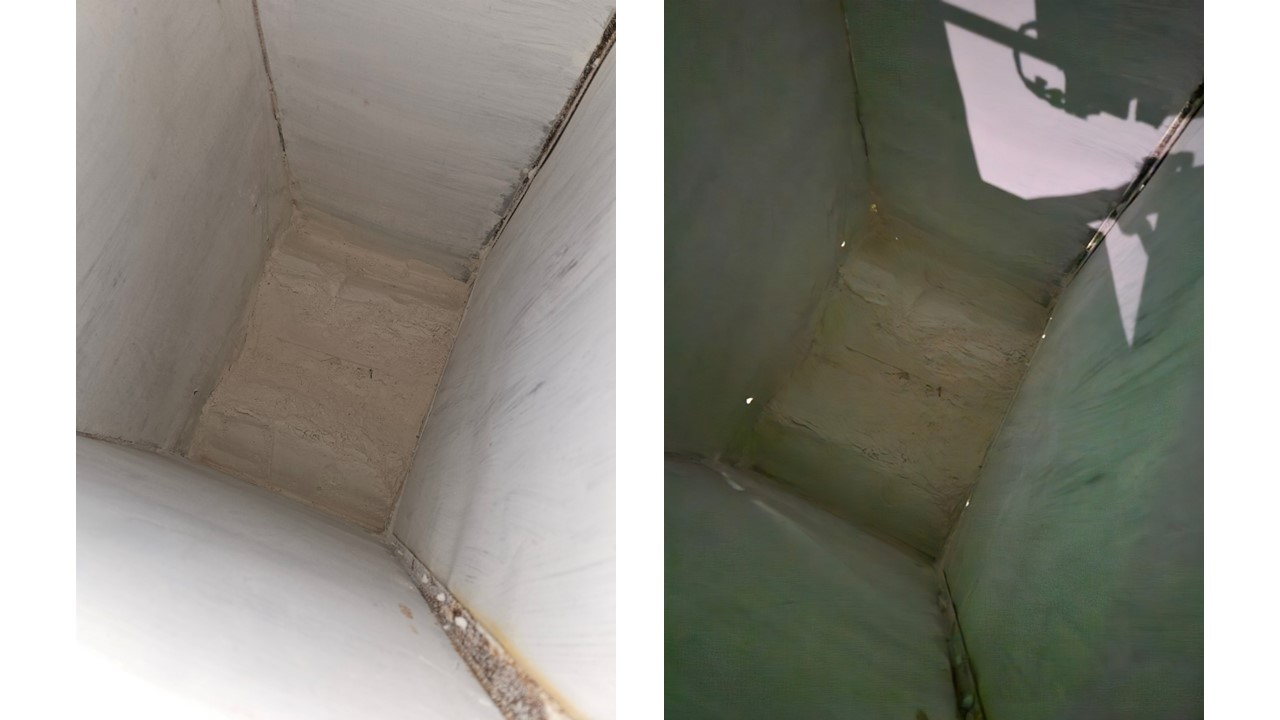
\includegraphics[width=1\textwidth]{Figures/test3-2-actual}
	\caption*{Actual Contour of 2}
\end{figure}

\newpage

\begin{center}
	\textbf{APPENDIX B (Contd.)}
\end{center}

\textbf{CONTOUR 3}

\begin{figure}[H]
	\centering
	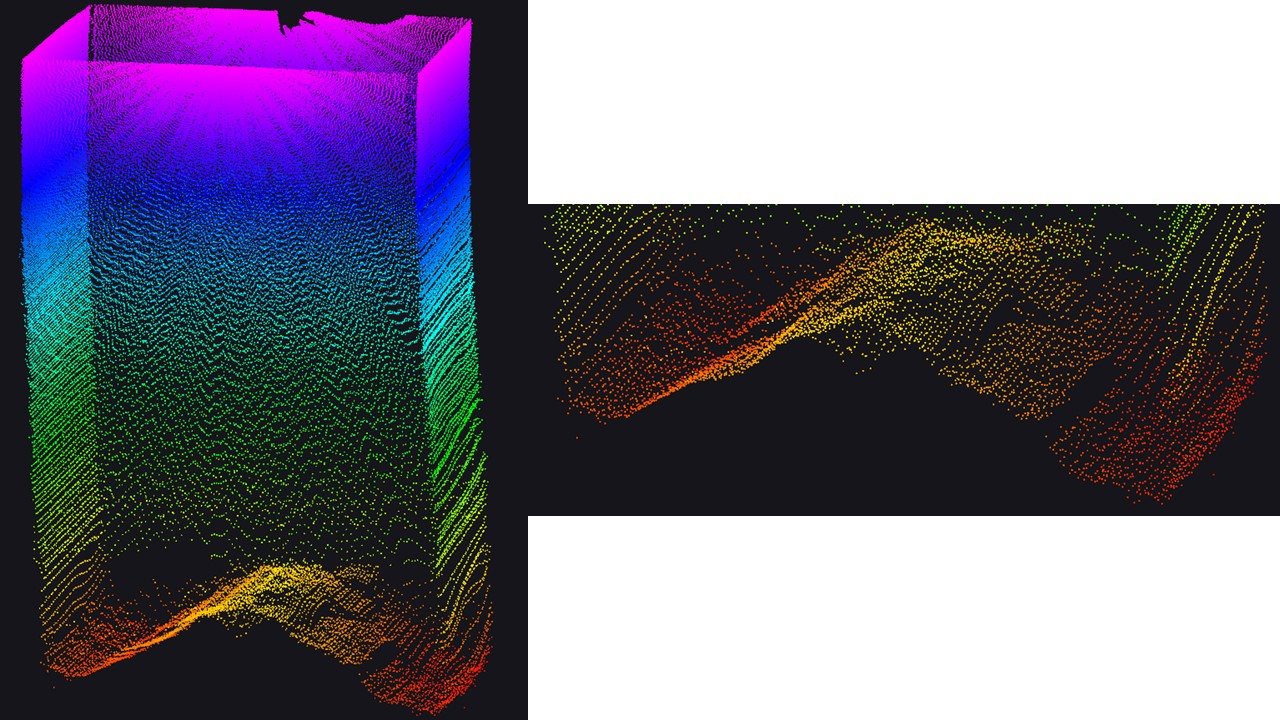
\includegraphics[width=1\textwidth]{Figures/test3-3}
	\caption*{3D Point Cloud of Contour 3}
\end{figure}

\vspace{0.5cm}

\begin{figure}[H]
	\centering
	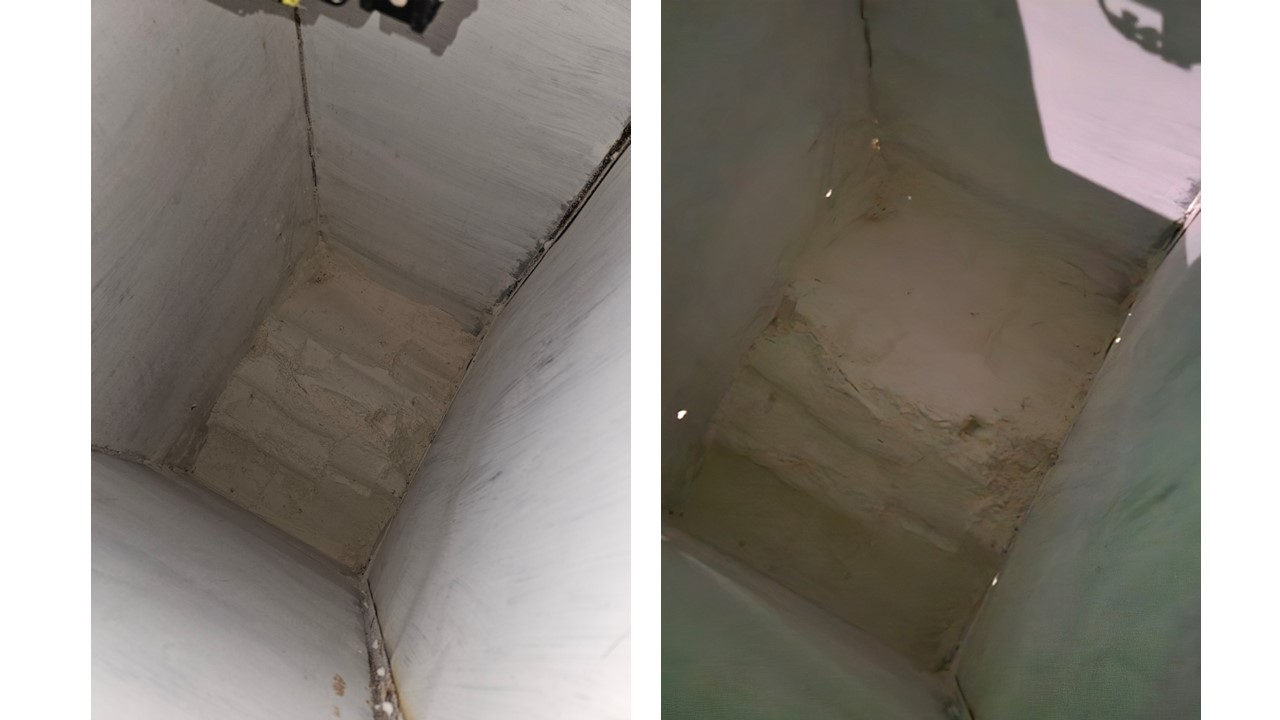
\includegraphics[width=1\textwidth]{Figures/test3-3-actual}
	\caption*{Actual Contour of 3}
\end{figure}

\newpage

\begin{center}
	\textbf{APPENDIX B (Contd.)}
\end{center}

\textbf{CONTOUR 4}

\begin{figure}[H]
	\centering
	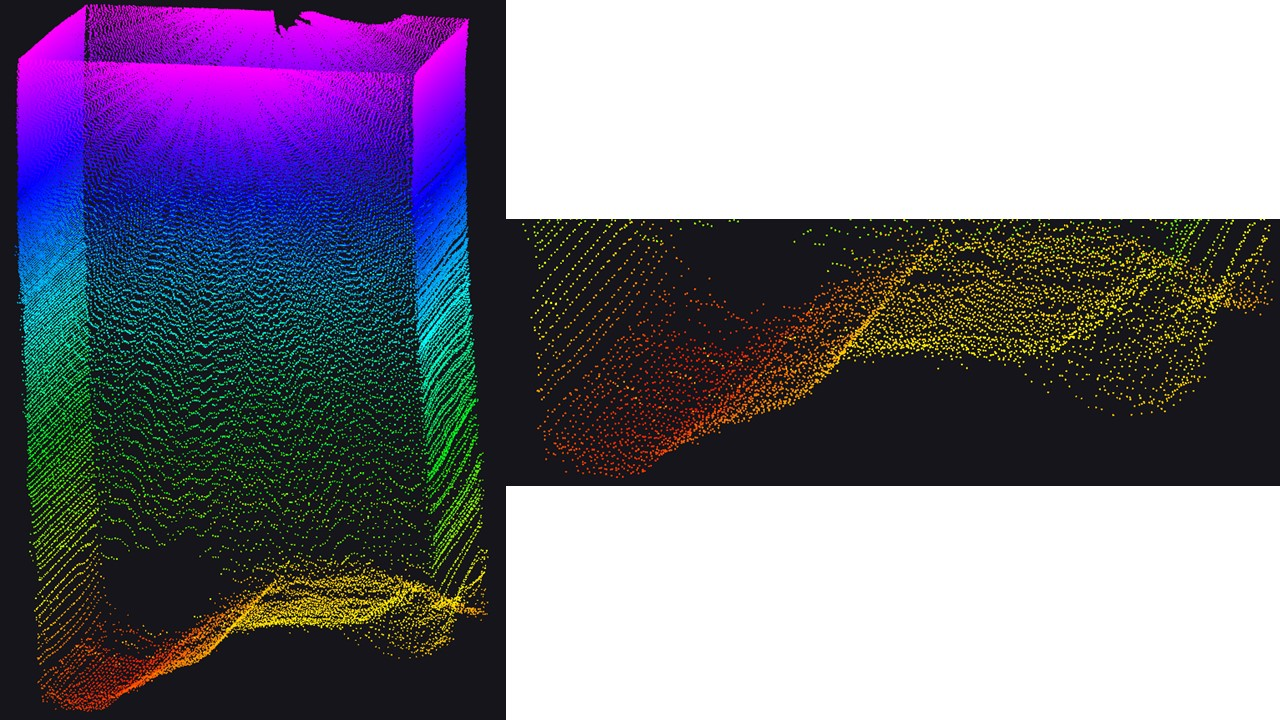
\includegraphics[width=1\textwidth]{Figures/test3-4}
	\caption*{3D Point Cloud of Contour 4}
\end{figure}

\vspace{0.5cm}

\begin{figure}[H]
	\centering
	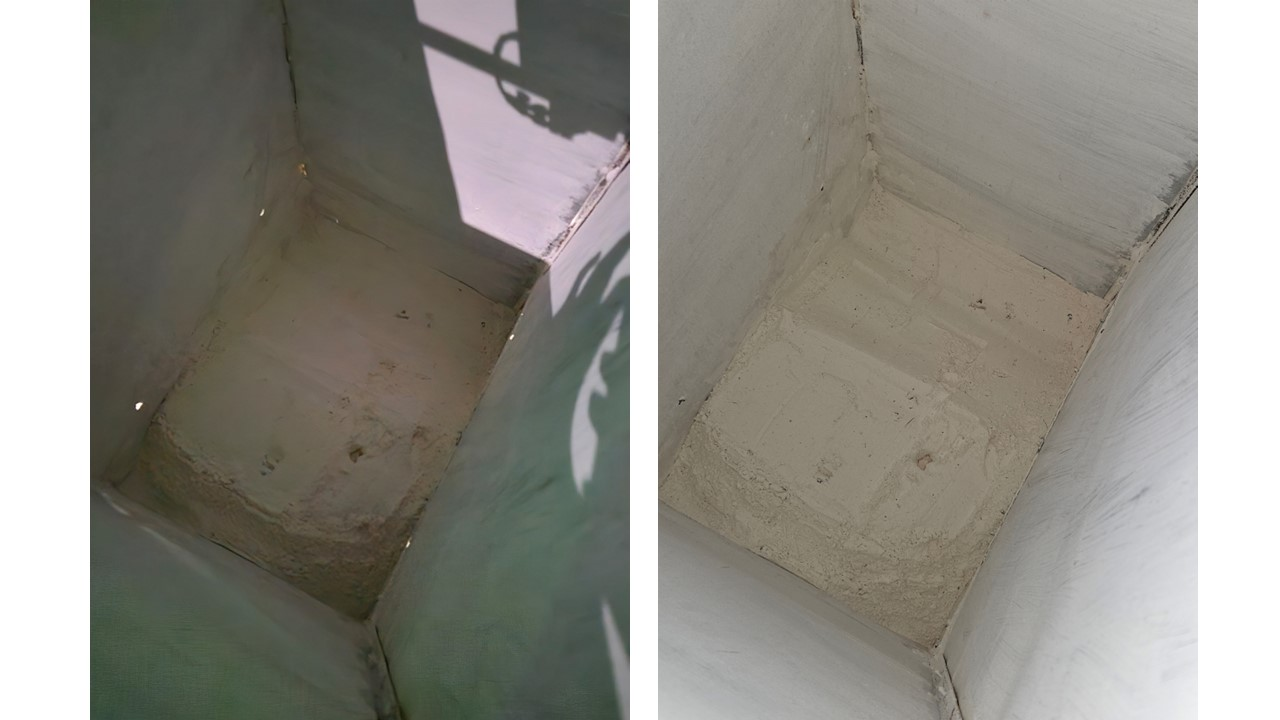
\includegraphics[width=1\textwidth]{Figures/test3-4-actual}
	\caption*{Actual Contour of 5}
\end{figure}

\newpage

\begin{center}
	\textbf{APPENDIX B (Contd.)}
\end{center}

\textbf{CONTOUR 5}

\begin{figure}[H]
	\centering
	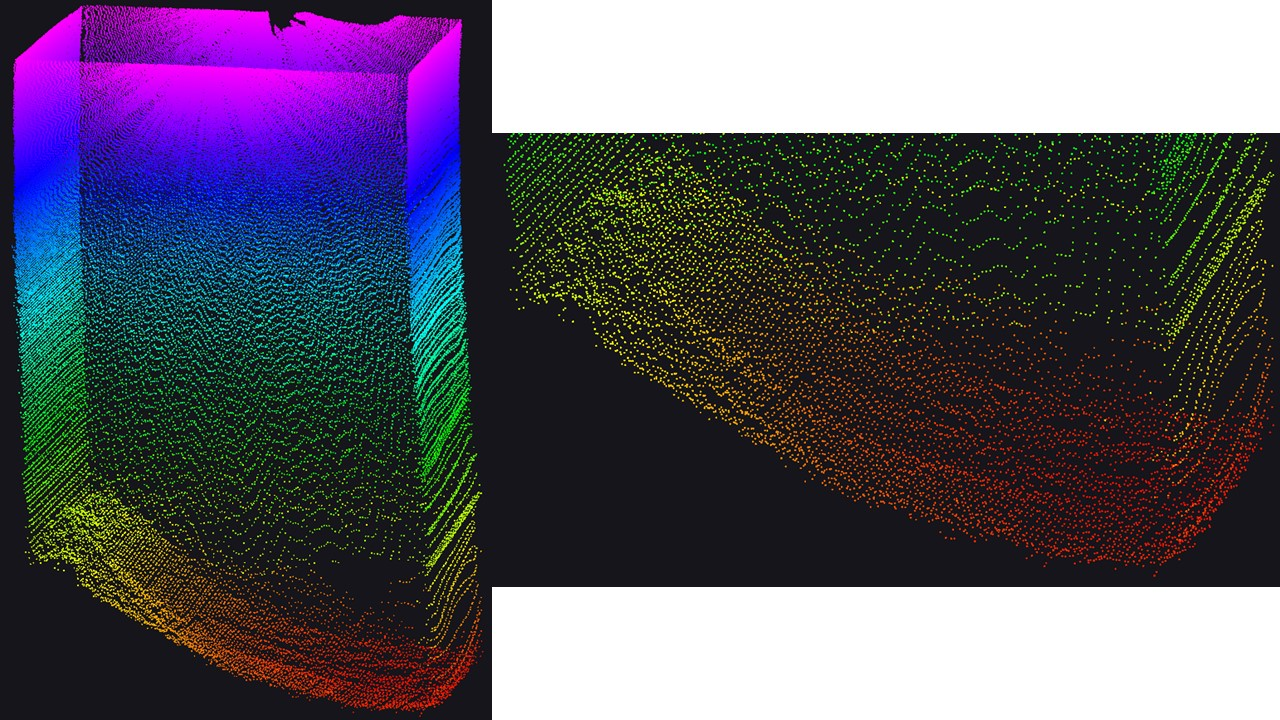
\includegraphics[width=1\textwidth]{Figures/test3-5}
	\caption*{3D Point Cloud of Contour 5}
\end{figure}

\vspace{0.5cm}

\begin{figure}[H]
	\centering
	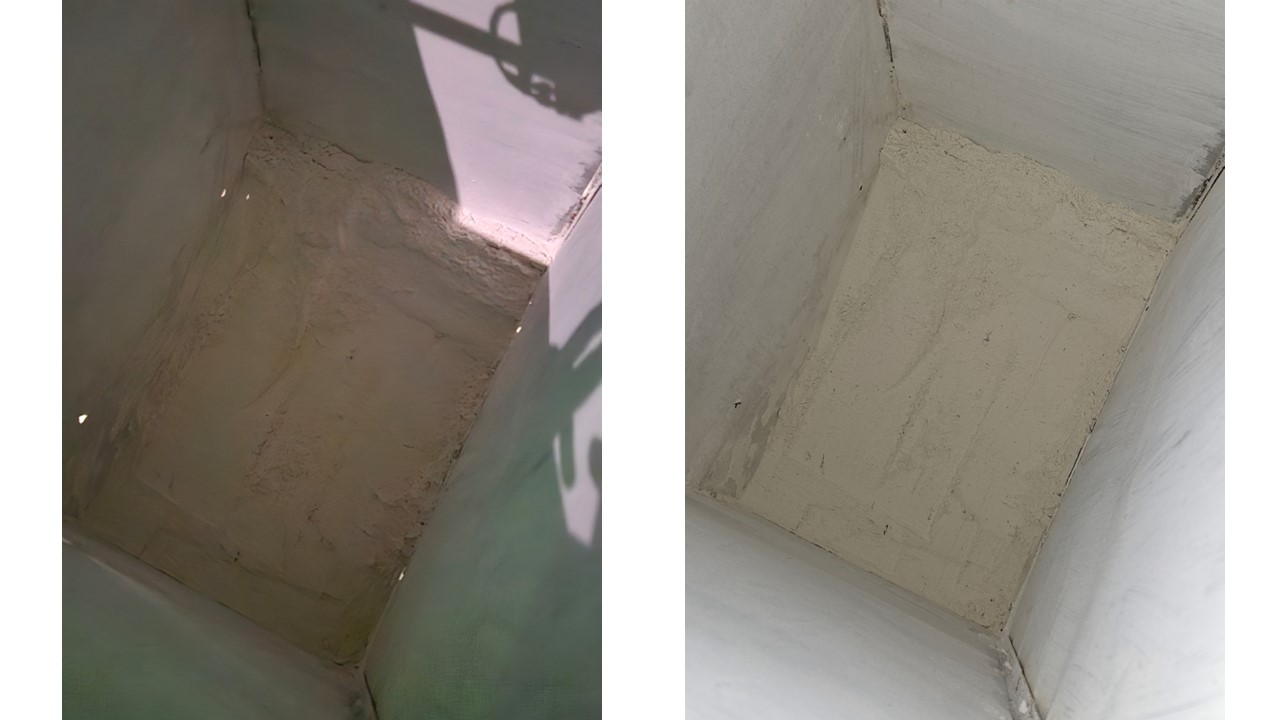
\includegraphics[width=1\textwidth]{Figures/test3-5-actual}
	\caption*{Actual Contour of 5}
\end{figure}

\newpage

\begin{center}
	\textbf{APPENDIX B (Contd.)}
\end{center}

\textbf{SOUNDING METHOD}

\begin{figure}[H]
	\centering
	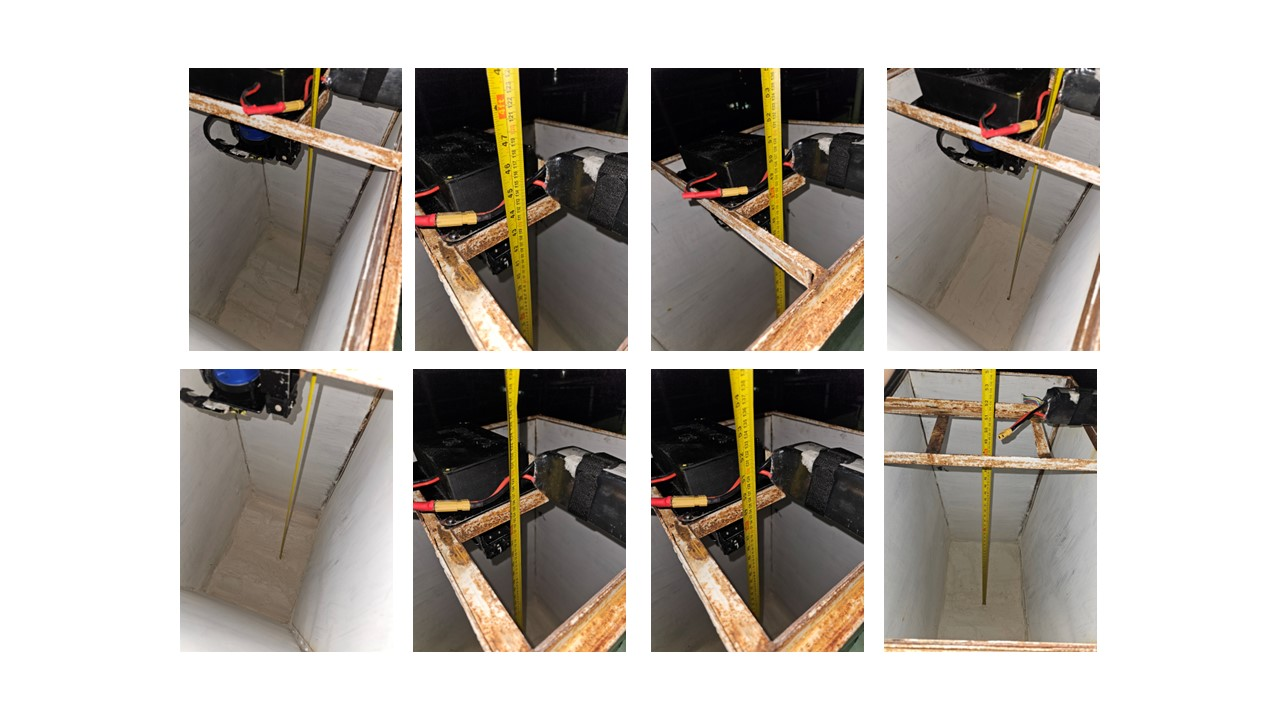
\includegraphics[width=1\textwidth]{Figures/test3-traditional}
	\caption*{Actual Sounding Method Testing}
\end{figure}